\documentclass{article}
\author{Jakub Muzyka i Jacek Paździerkiewicz}
\title{Raport nr 1 z przedmiotu:\\ "Symulacje komputerowe"\\ Temat: Generowanie zmiennych losowych różnymi metodami}
\date{\today}
\usepackage{geometry}
\usepackage{graphicx} 
\usepackage{float}
\setlength{\abovecaptionskip}{10pt}
\setlength{\belowcaptionskip}{10pt}
\usepackage{subfigure}
\renewcommand*{\figurename}{Wykres}
\newgeometry{tmargin=1cm, bmargin=2.0cm, lmargin=1.5cm, rmargin=1.5cm}
\usepackage[T1]{fontenc}
\parskip 0.4 cm
\usepackage{amsmath}
\begin{document}
	\maketitle
	\large
	\textbf{Czym są liczby pseudolosowe?}
	
	\textbf{Liczbami pseudolosowymi} są liczby wyglądające jak losowe, które tworzy się algorytmicznie. Dzięki temu, znając tylko kilka kolejnych liczb pseudolosowych, możemy wygenerować wszystkie następne.
	
	W naszym raporcie przedstawimy różne sposoby generowania zmiennych losowych:
	\begin{enumerate}
		\item \textbf{Metoda odwrotnej dystrybuanty dla rozkładów dyskretnych} \\
		
		Chcemy wygenerować wartość z rozkładu dyskretnego o prawdopodobieństwie $$P(X=x_{j}) = p_{j},\hspace{1em}j=0,1,\ldots,\sum_j p_{j} = 1$$
		Żeby osiągnąć nasz cel, musimy generować zmienną $U\sim (0,1)$ z rozkładu jednostajnego i odpowiednio zwracać wartość p, jeżeli $U$ spełnia warunek nierówności:
		$$\left\{
		\begin{array}{ccccc}
			x_{0}&if~U < p_{0}\\
			x_{1}&if~p_{0}\le U<p_{0} + p_{1}\\
			\vdots\\
			x_{j}& if~\sum_{i=0}^{j-1} p_{i}\le U < \sum_{i=0}^{j} p_{i}\\
			\vdots
		\end{array}
		\right.$$
		Wiemy, że kiedy $0<a<b<1$ mamy $P(a\le U < b) = b-a$, to:
		$$P(X = x_{j}) = P(\sum_{i=0}^{j-1} p_{i}\le U < \sum_{i=0}^{j} p_{i}) = p_{j}$$ Jest naszą szukaną dystrybuantą.
		
		\textbf{Algorytm:}
		\begin{enumerate}
			\item Generuj $U\sim (0,1)$
			\item Jeżeli $U < p_{0}~ \text{zwróć}~X=x_{0}~ \text{i kończymy program}$
			\item Jeżeli $U < p_{0} + p_{1}~\text{zwróć}~X=x_{1}~\text{i kończymy program}$
			\item Jeżeli $U < p_{0} + p_{1} + p_{2}~\text{zwróć}~X=x_{2}~\text{i kończymy program}\ldots etc.$
		\end{enumerate}
		\textbf{Przykładowa implementacja:}
		
		Weźmy rozkład dyskretny z konkretnymi prawdopodobieństwami:
		$$P(X = 1) = 0.2, P(X = 2) = 0.15, P(X = 3) = 0.35, P(X = 4) = 0.3$$
		Które zgodnie z definicją prawdopodobieństwa sumują się do 1.  
		\begin{figure}[h]
			\begin{center}
				\subfigure{
					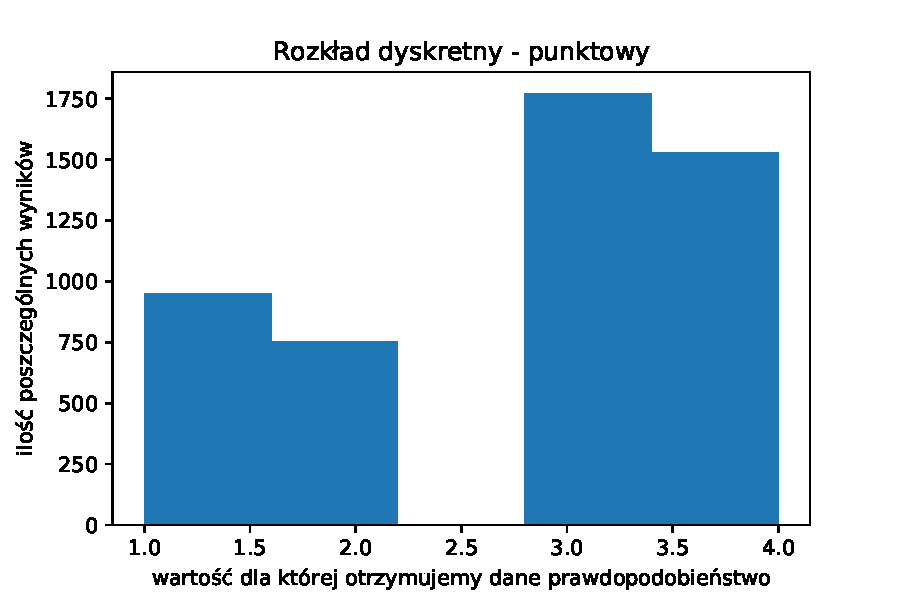
\includegraphics[width=8cm]{obrazek1a.pdf}
				}
				\subfigure{
					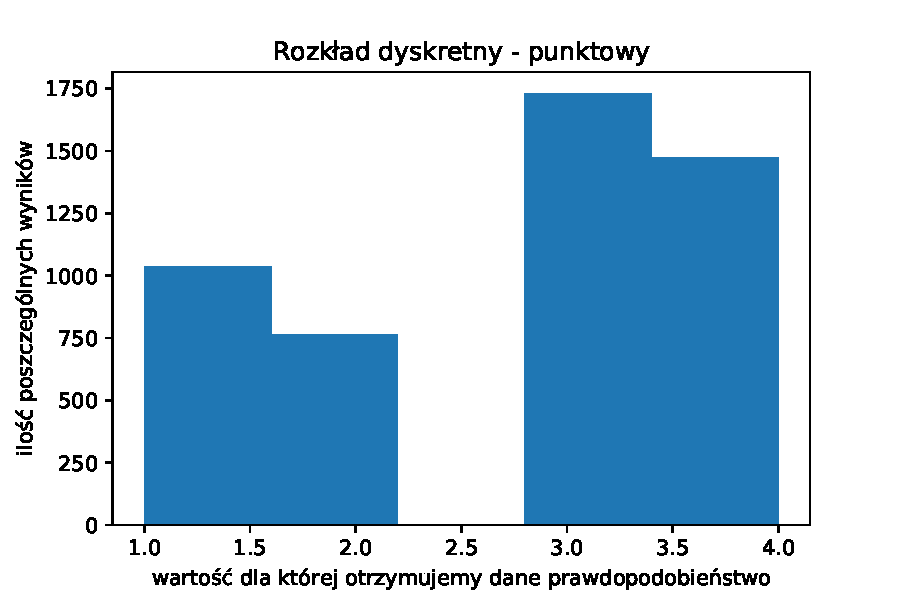
\includegraphics[width=8cm]{obrazek1b.pdf}
				
				}
				\caption{dla 1000 losowań}
				\caption{dla 5000 losowań}
			\end{center}
		\end{figure}
	
		Wykonujemy również test empiryczny dla dystrybuanty naszego rozkładu:
		\begin{figure}[h]
			\begin{center}
				\subfigure{
					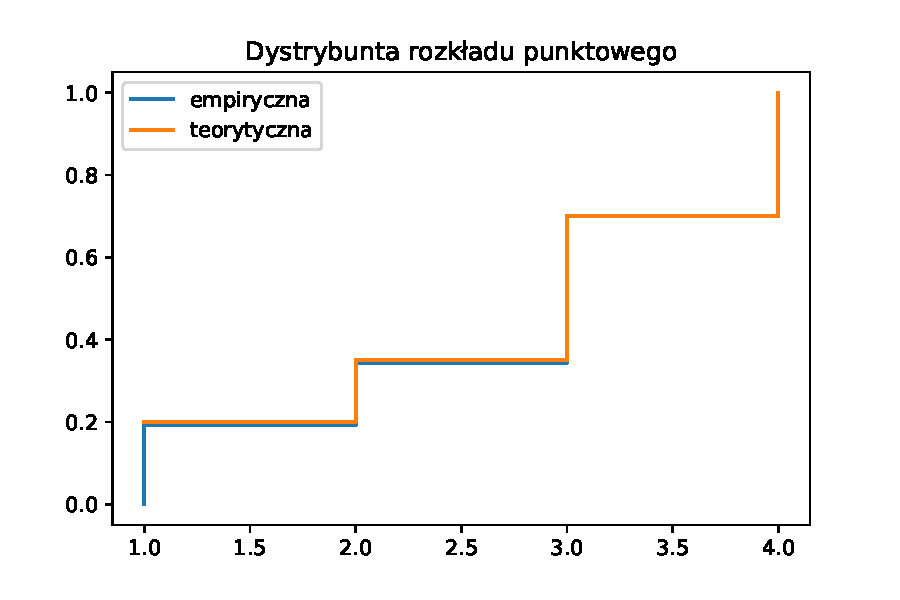
\includegraphics[width=8cm]{obrazek2a.pdf}
				}
				\subfigure{
					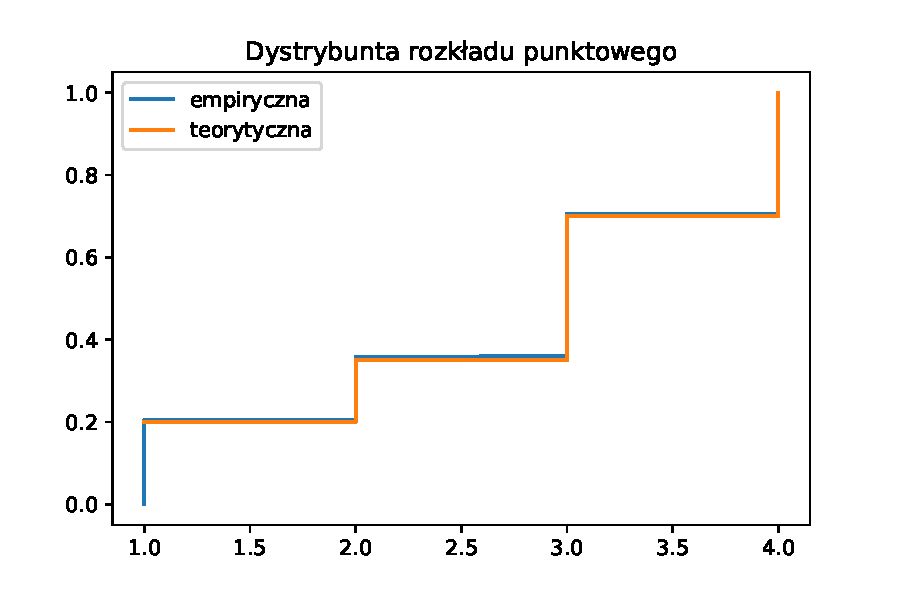
\includegraphics[width=8cm]{obrazek2b.pdf}
					
				}
				\caption{dla 1000 losowań}
				\caption{dla 5000 losowań}
			\end{center}
		\end{figure}
		
		Widzimy, że zarówno dystrybuanta empiryczna, jak i teoretyczna pokrywają się,a to oznacza, że nasza metoda odwrotnej dystrybuanty dla rozkładów dyskretnych jest poprawnie zaimplementowana.
		
		\item \textbf{Metoda odwrotnej dystrybuanty dla rozkładów ciągłych}\\
		
		Dążymy do tego, żeby wyprowadzić dystrybuantę odwrotną ze wzoru $u = F(X)$:
		$$X = F^{-1}(U);\hspace{1em} U(0,1)$$ 
		\textbf{Algorytm:}
		\begin{enumerate}
			\item Generuj $U\sim (0,1)$
			\item Znajdź $x = F^{-1}(U)$ dla $u = F(x)$
			\item 
			Wstaw $u$ do $x = F^{-1}(U)$ i zwróć wartość
		\end{enumerate}
		\textbf{Przykładowe implementacje:}
		Użyjemy rozkładu Pareto, które gęstość i dystrybuanta wyglądają następująco:
		$$f(x) = \alpha(\frac{\lambda}{x})^\alpha\frac{1}{x}$$
		$$ F(x) = 1 - (\frac{\lambda}{x})^\alpha$$
		Na początek porównujemy gęstość empiryczną i teoretyczną tego rozkładu:
		\begin{figure}[h]
			\begin{center}
				\subfigure{
					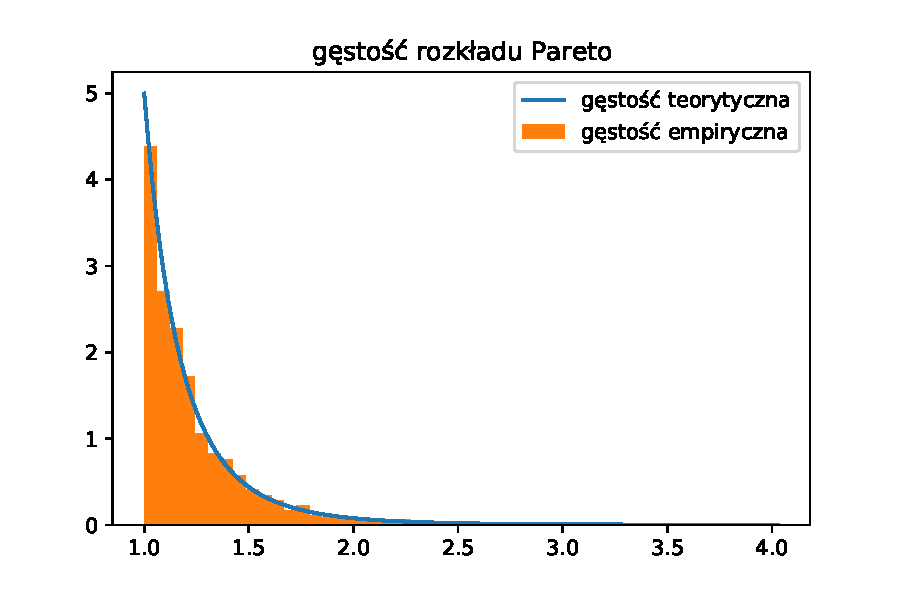
\includegraphics[width=8cm]{obrazek3a.pdf}
				}
				\subfigure{
					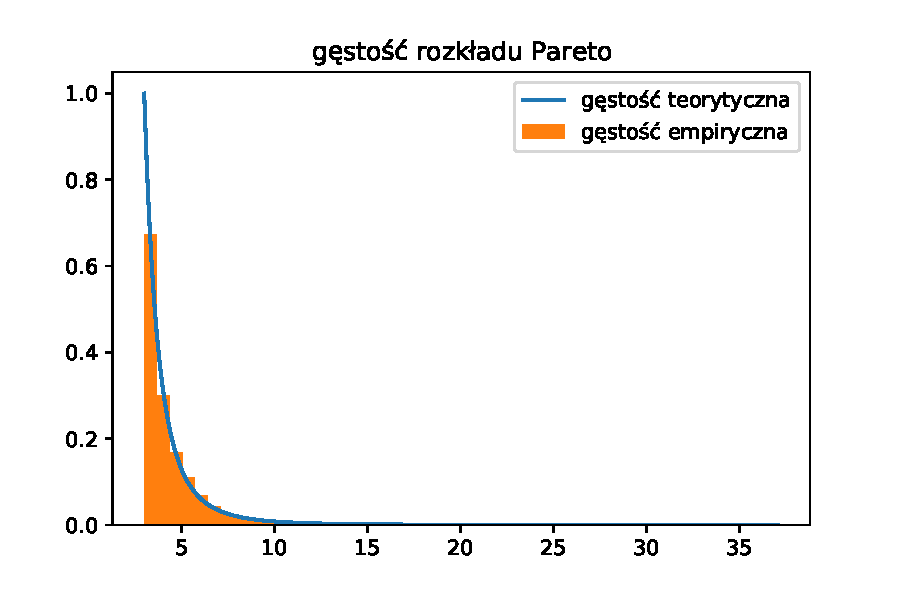
\includegraphics[width=8cm]{obrazek3b.pdf}
					
				}
				\caption{dla $\alpha = 5$,$\lambda = 1$ i dla 1000 losowań}
				\caption{dla $\alpha = 3$,$\lambda = 3$ i dla 3000 losowań}
			\end{center}
		\end{figure}
	
		A następnie to samo dla dystrybuanty:
		\begin{figure}[h]
			\begin{center}
				\subfigure{
					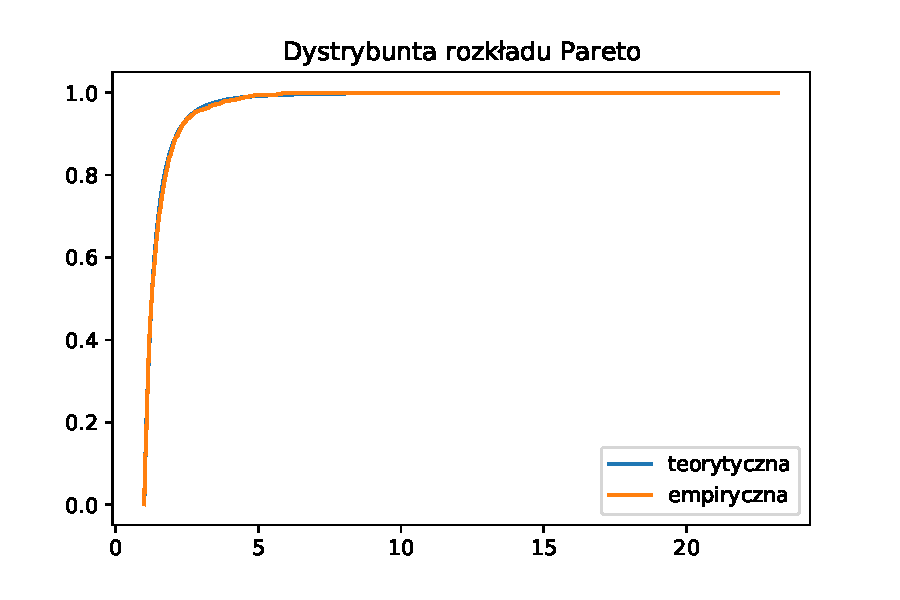
\includegraphics[width=8cm]{obrazek4a.pdf}
				}
				\subfigure{
					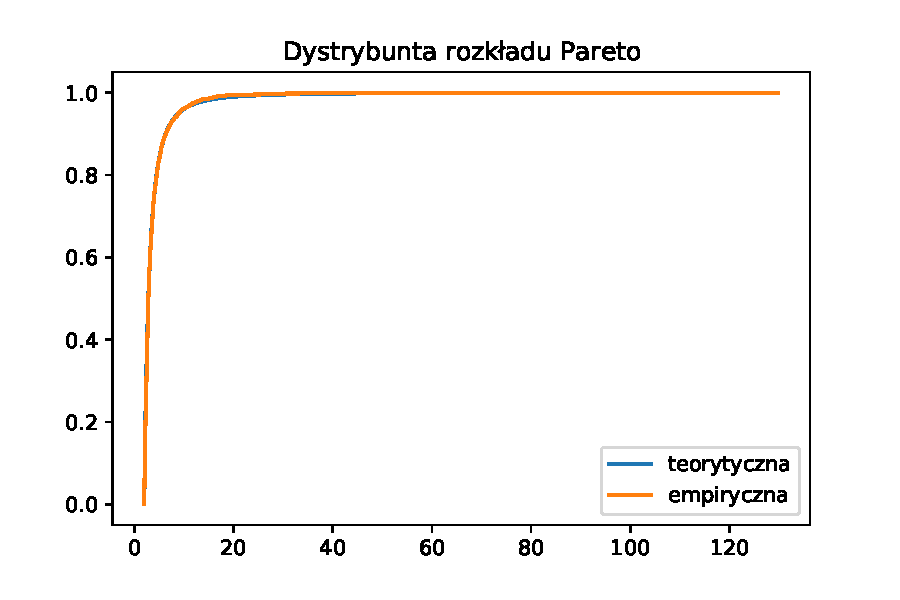
\includegraphics[width=8cm]{obrazek4b.pdf}
					
				}
				\caption{dla $\alpha = 3$,$\lambda = 1$ i dla 1000 losowań}
				\caption{dla $\alpha = 2$,$\lambda = 2$ i dla 3000 losowań}
			\end{center}
		\end{figure}
	
		Dla sprawdzenia poprawności naszej metody implementujemy wbudowany rozkład Pareto:
		
		\begin{figure}[h]
			\centering
			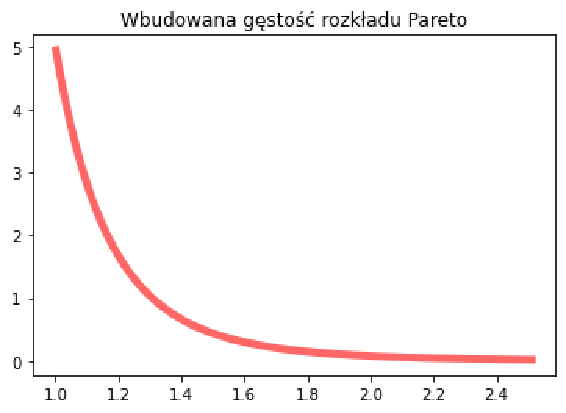
\includegraphics{obrazek5.pdf}
		\end{figure}
	
		\textbf{Wnioski:} 
		
		Możemy zauważyć, że zarówno gęstość teoretyczna i wbudowana rozkładu Pareto, przechodzą przez te same punkty. Dodatkowo dystrybuanta empiryczna i teoretyczna, pokrywają się, co świadczy o poprawnej implementacji naszej metody. 
		
		\item \textbf{Metoda kompozycji}\\
		
		Jeśli wiemy, że jesteśmy w stanie wyznaczyć dystrybuanty zmiennych losowych $Y_{i}$ równych $F_{i},\hspace{0.5em} i=1,2,3,..$, to zakładamy, że zmienna X ma dystrybuantę postaci:
		$$F_{X}(x) = \sum_{i=1}^{n} p_{i}F_{i}(x),\hspace{1em}\text{gdzie}~p_{i} > 0, \sum_{i=1}^{n} p_{i} = 1$$ oraz $F_{i}$, to dystrybuanty pewnych zmiennych losowych $Y_{i}$.
		
		Jeśli $X,Y_{1},\ldots,Y_{n}$ mają gęstości, to wyżej wymieniony wzór można równoważnie zapisać:
		$$f_{x}(x) = \sum_{i=1}^{n}p_{i}f_{i}(x)$$
		\textbf{Algorytm dla rozkładu ciągłego:}
		\begin{enumerate}
			\item Generuj zmienną losową z rozkładu jednostajnego $U\sim(0,1)$
			\item Przy pomocy metody odwrotnej dystrybuanty wyznacz wybrany rozkład jako funkcję z naszą losową wartością $U\sim(0,1)$
			\item zmieniaj losowo znak funkcji 
			\item zwróć wartość funkcji 
		\end{enumerate}
		\textbf{Przykładowe implementacje:}
		
		Użyjemy rozkładu Laplace'a, który jest różnicą dwóch rozkładów wykładniczych z gęstością i dystrybuantą daną wzorem:
		$$f(x) = \frac{\lambda}{2}e^{-\lambda|x|}$$
		$$F(x) = \frac{1}{2} + \frac{1}{2}sgn(x)(1 - e^{-|x|})$$
		Komponujemy rozkład Laplace'a z dwóch rozkładów wykładniczych i porównujemy jego gęstość oraz dystrybuantę empiryczną i teoretyczną:
		\begin{figure}[h]
			\begin{center}
				\subfigure{
					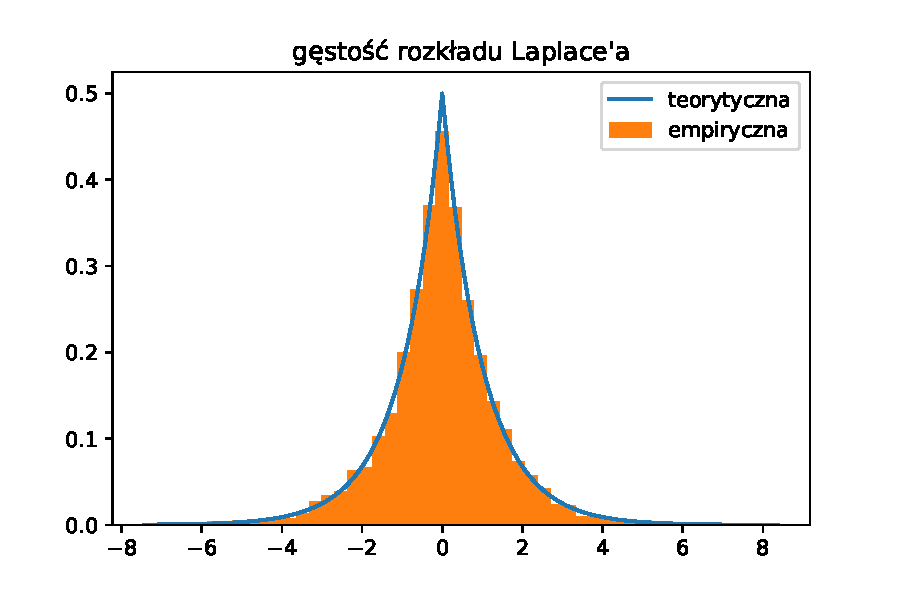
\includegraphics[width=8cm]{obrazek5a.pdf}
				}
				\subfigure{
					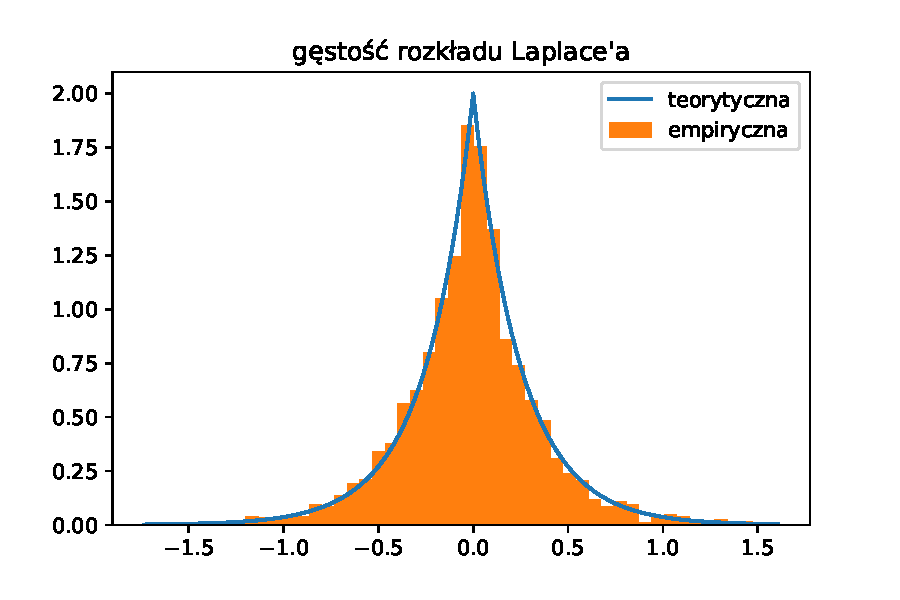
\includegraphics[width=8cm]{obrazek5b.pdf}
					
				}
				\caption{dla $\lambda = 1$ i dla 5000 losowań}
				\caption{dla $\lambda = 4$ i dla 3000 losowań}
			\end{center}
		\end{figure}
		\begin{figure}[h]
			\begin{center}
				\subfigure{
					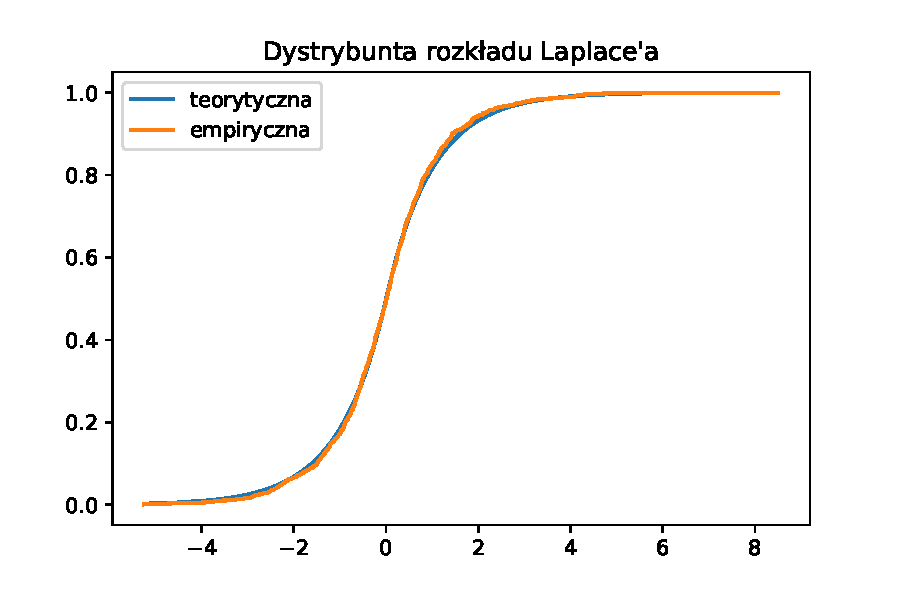
\includegraphics[width=8cm]{obrazek6a.pdf}
				}
				\subfigure{
					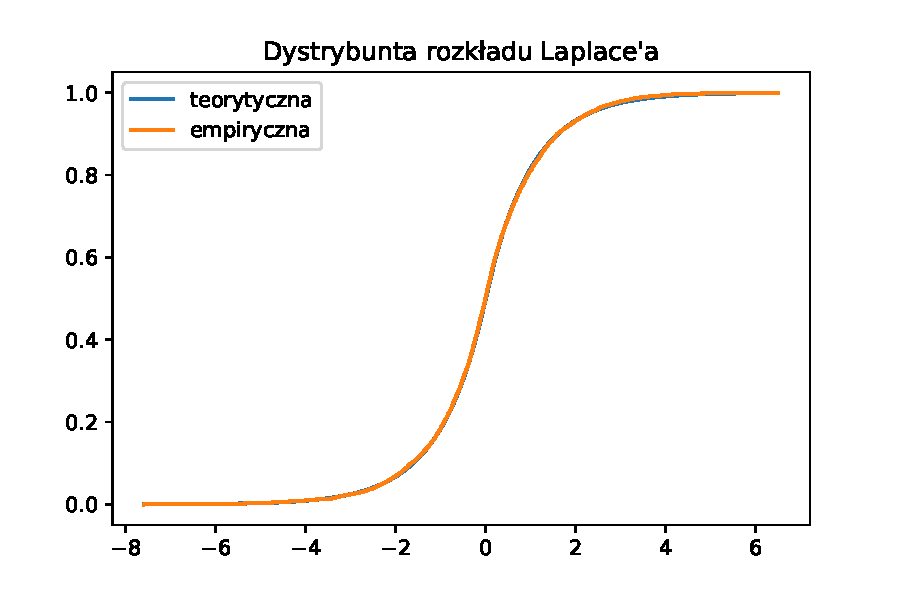
\includegraphics[width=8cm]{obrazek6b.pdf}
					
				}
				\caption{dla 1000 losowań}
				\caption{dla 5000 losowań}
			\end{center}
		\end{figure}
	
		Dodatkowo, w ramach ciekawostki stworzyliśmy 'gładki' estymator gęstości teoretycznej:
		
		\begin{figure}[H]
			\centering
			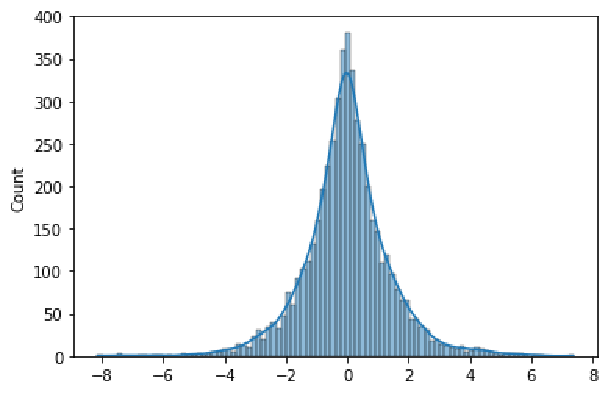
\includegraphics{obrazek8.pdf}
		\end{figure}
		
		\textbf{Wnioski:}
		
		Tak jak w poprzednich przykładach, widzimy, że gęstości oraz dystrybuanty pokrywają się, dlatego metoda kompozycji dla rozkładu ciągłego — Laplace'a, jest poprawnie zaimplementowana.
		
		\item \textbf{Metoda Boxa - M{\"u}llera}\\
		
		Metoda ta opiera się na losowaniu wartości z rozkładu jednostajnego i podstawieniu do zdefiniowanych rozkładów X i Y:
		$$X = \sqrt{-2\log(U_{1})}\cos(2\pi U_{2})$$
		$$Y = \sqrt{-2\log(U_{1})}\sin(2\pi U_{2})$$
		Wtedy otrzymujemy, że X i Y są niezależne i mają takie same rozkłady, oraz $X,Y \sim N(0,1)$.
		Wyznaczyliśmy te zmienne ze współrzędnych biegunowych, niezależnych zmiennych X i Y:
		$$ R^2 = X^2 + Y^2$$
		$$ \tan{\theta} = \frac{Y}{X}$$
		,gdzie $X = R\cos{\theta}, Y = R\sin{\theta}$, a gęstość łączna, to złożenie dwóch niezależnych rozkładów normalnych dla $X, Y \sim N(0,1)$, czyli:
		$$ f(x,y) = \frac{1}{2\pi}e^{-\frac{(x^2 + y^2)}{2}}$$
		
		\textbf{Algorytm:}
		\begin{enumerate}
			\item Generuj $U_{1}\sim U(0,1),U_{2}\sim U(0,1)$ 
			\item Wstaw $X = \sqrt{-2\log(U_{1})}\cos(2\pi U_{2})$,\hspace{1em}$Y = \sqrt{-2\log(U_{1})}\sin(2\pi U_{2})$
		\end{enumerate}
		\textbf{Przykładowe implementacje:}
		
		Analizę naszych danych zaczęliśmy od porównania, wyprowadzonych już, dwóch gęstości, wyznaczonych metodą odwrotnej dystrybuanty:
		\begin{figure}[h]
			\begin{center}
				\subfigure{
					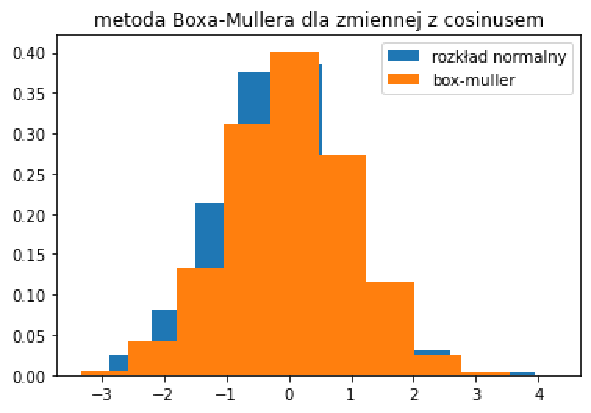
\includegraphics[width=8cm]{obrazek9.pdf}
				}
				\subfigure{
					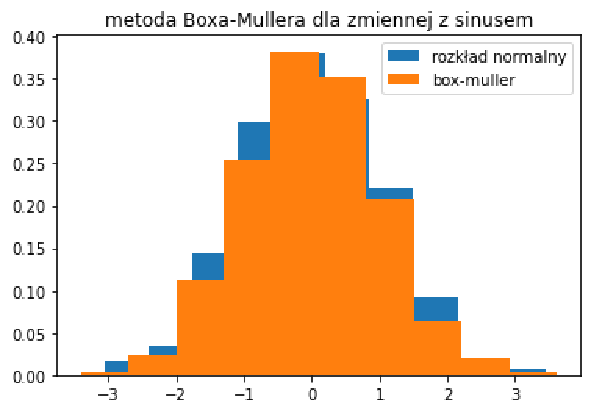
\includegraphics[width=8cm]{obrazek10.pdf}
				}
			\caption{dla 1000 losowań}
			\end{center}
		\end{figure} 
	
		\begin{figure}[h]
			\begin{center}
				\subfigure{
					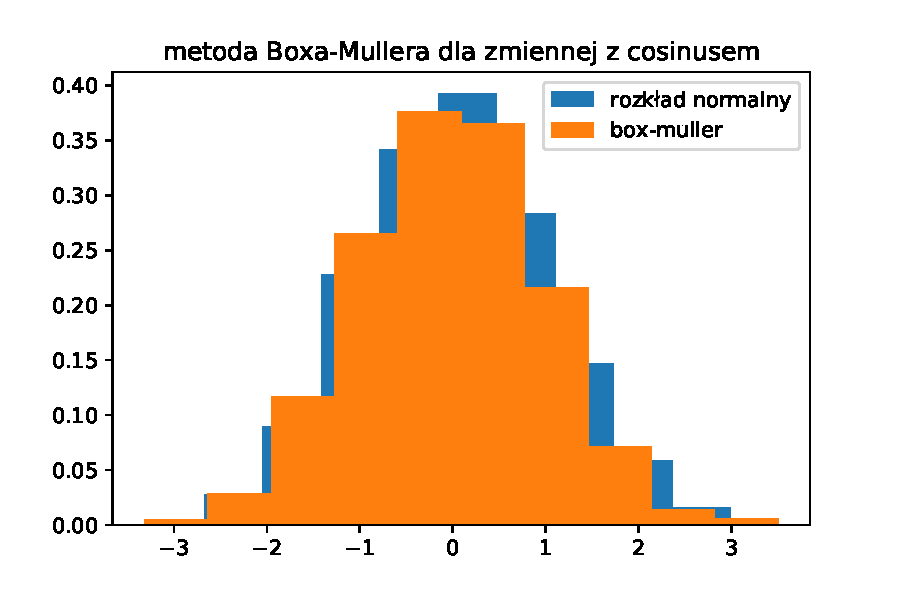
\includegraphics[width=8cm]{obrazek10a.pdf}
				}
				\subfigure{
					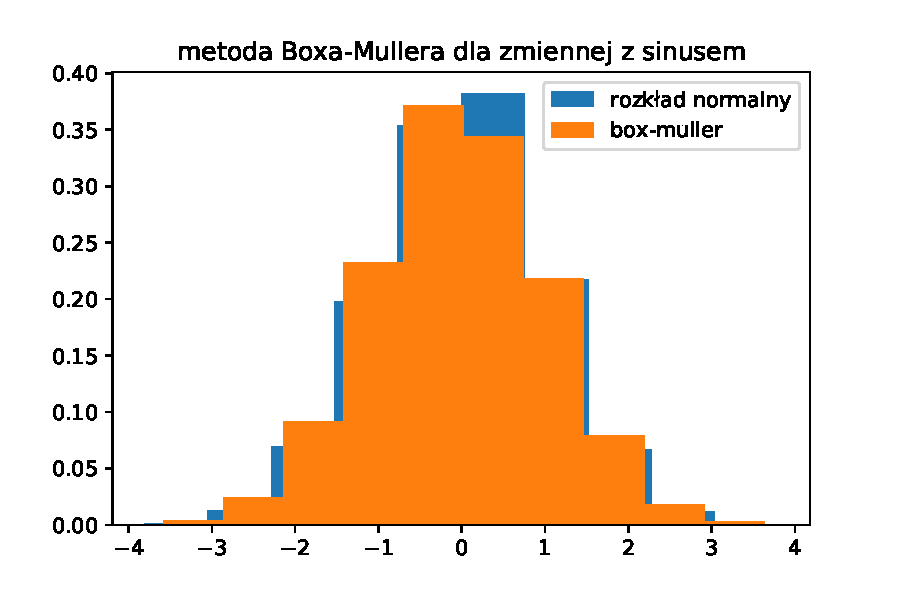
\includegraphics[width=8cm]{obrazek10b.pdf}
				}
				\caption{dla 5000 losowań}
			\end{center}
		\end{figure}
	
		Następnie porównujemy gęstości każdej zmiennej z teoretyczną gęstością rozkładu normalnego:
		\begin{figure}[h]
			\begin{center}
				\subfigure{
					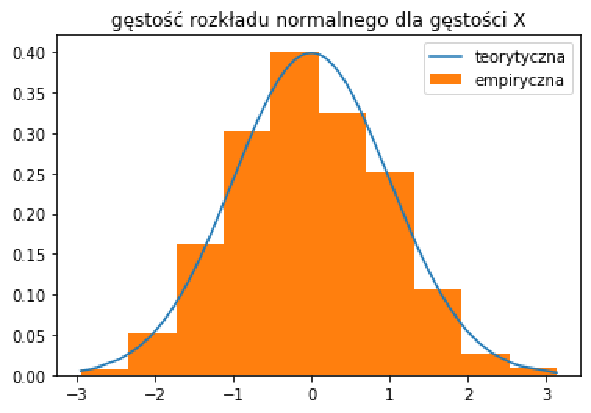
\includegraphics[width=8cm]{obrazek11.pdf}
				}
				\subfigure{
					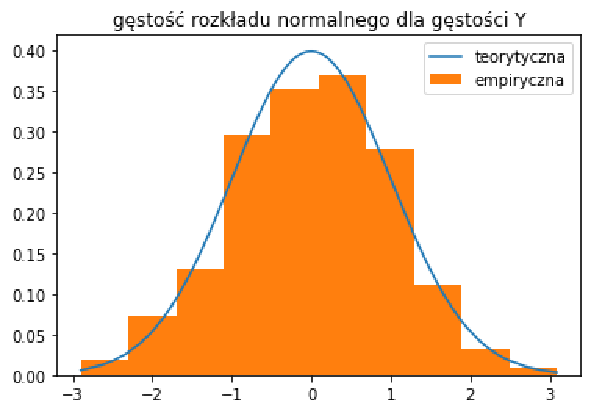
\includegraphics[width=8cm]{obrazek12.pdf}
				}
		
				\caption{dla 1000 losowań}
			\end{center}
		\end{figure} 
	
		\begin{figure}[h]
			\begin{center}
				\subfigure{
					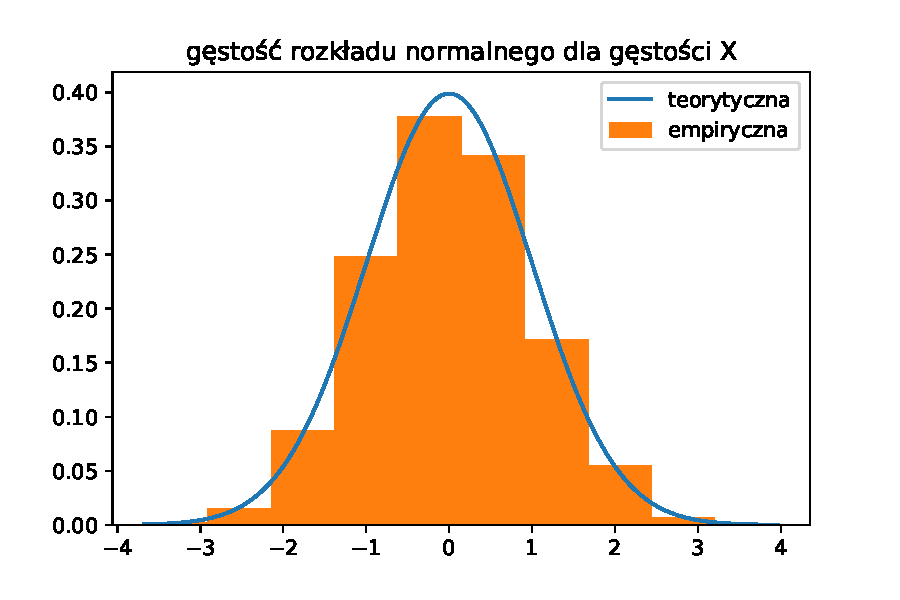
\includegraphics[width=8cm]{obrazek11a.pdf}
				}
				\subfigure{
					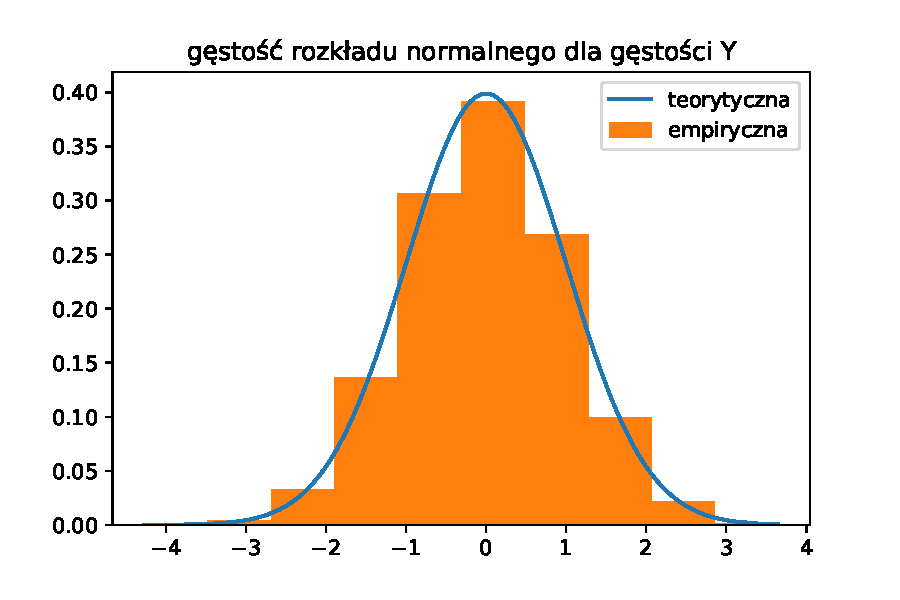
\includegraphics[width=8cm]{obrazek11b.pdf}
				}
				\caption{dla 5000 losowań}
			\end{center}
		\end{figure} 
	
		To samo dla dystrybuant:
		\begin{figure}[h]
			\begin{center}
				\subfigure{
					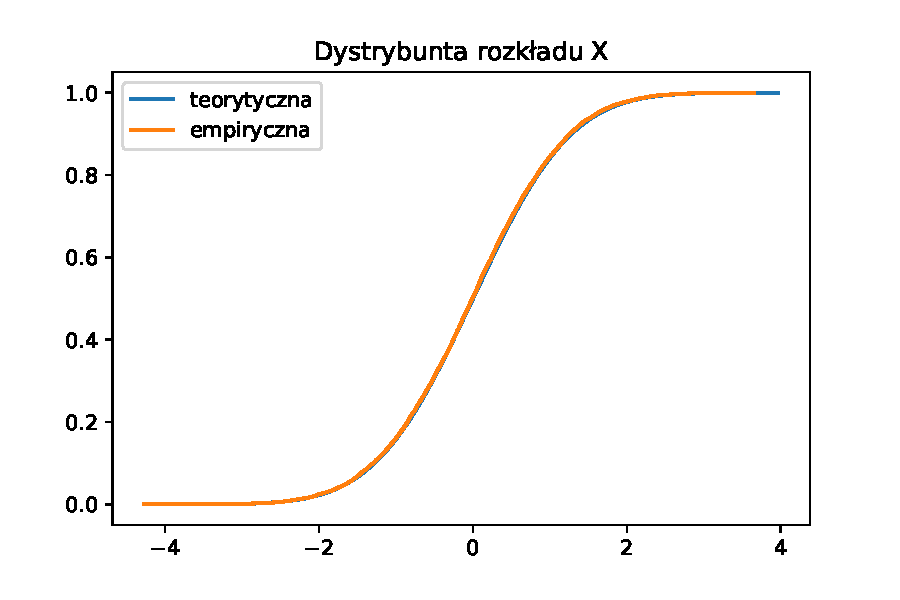
\includegraphics[width=8cm]{obrazek18a.pdf}
				}
				\subfigure{
					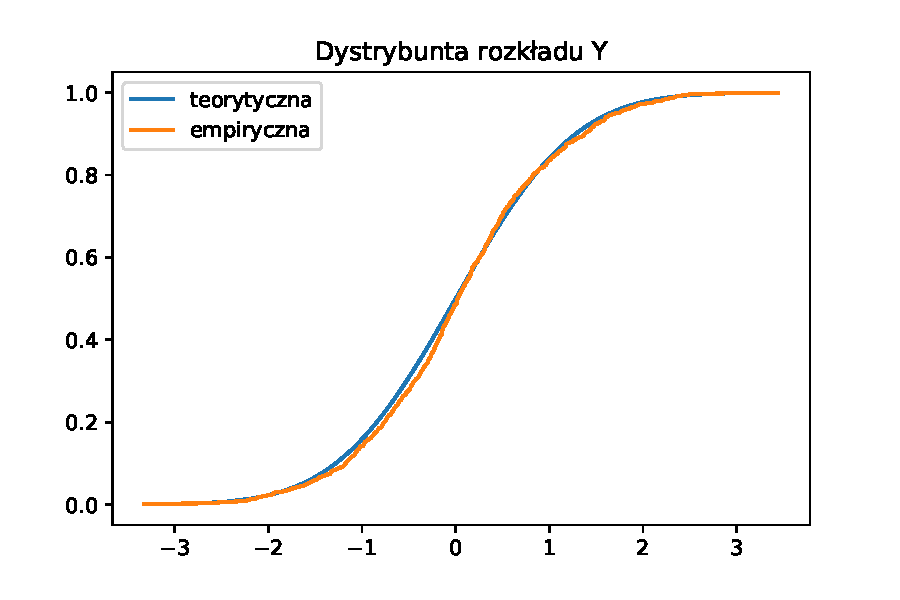
\includegraphics[width=8cm]{obrazek18b.pdf}
				}
				\caption{dla 5000 losowań}
			\end{center}
		\end{figure} 
		
		\begin{figure}[h]
			\begin{center}
				\subfigure{
					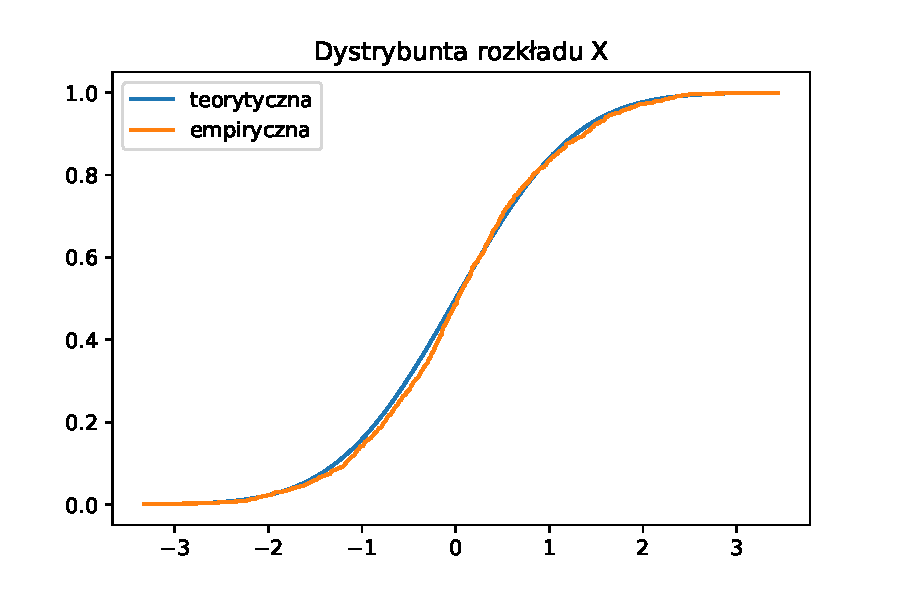
\includegraphics[width=8cm]{obrazek19a.pdf}
				}
				\subfigure{
					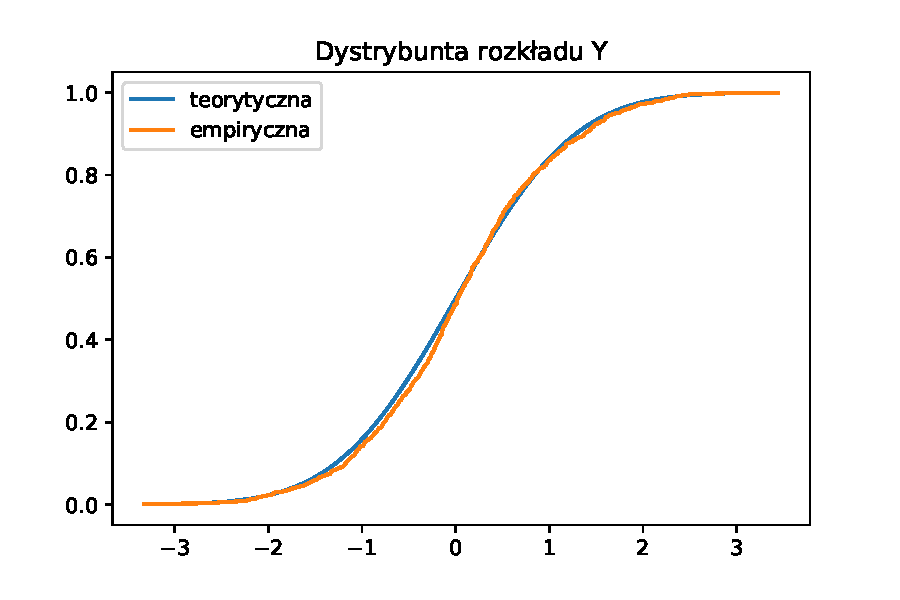
\includegraphics[width=8cm]{obrazek19b.pdf}
				}
				\caption{dla 1000 losowań}
			\end{center}
		\end{figure} 
	
		Dodatkowo implementujemy wbudowany rozkład normalny oraz QQ-plot'y dla wyznaczonych przez nas gęstości i dystrybuanty, w celu potwierdzenia poprawności naszej metody:
		\begin{figure}[h]
			\begin{center}
				\subfigure{
					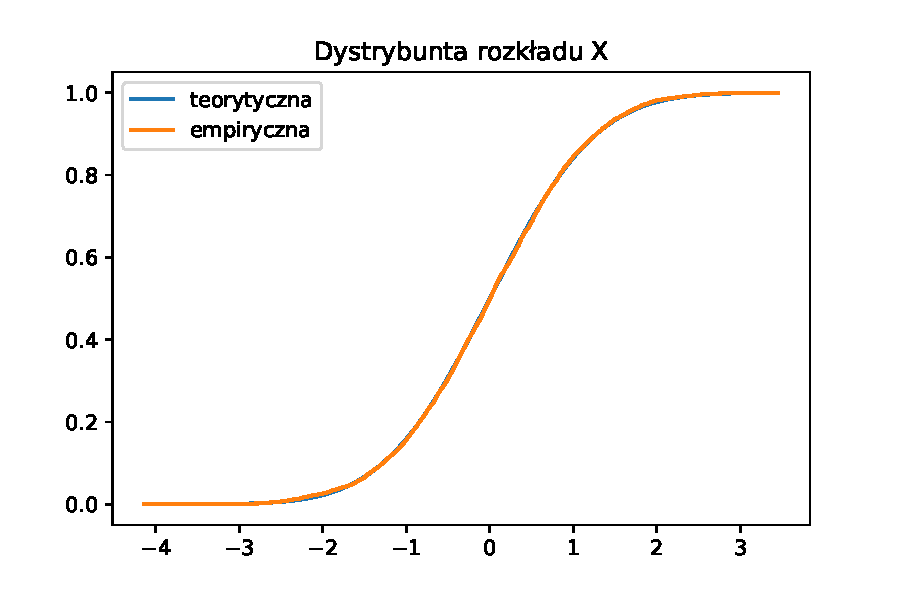
\includegraphics[width=8cm]{obrazek21a.pdf}
				}
				\subfigure{
					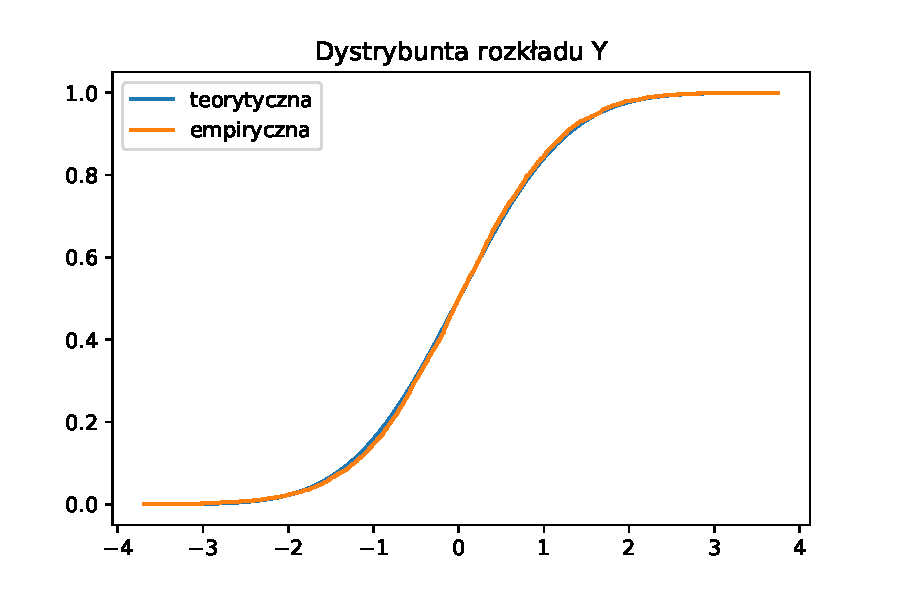
\includegraphics[width=8cm]{obrazek21b.pdf}
				}
				\caption{Gęstości X i Y dla 5000 losowań}
			\end{center}
		\end{figure}
	
		\begin{figure}[h]
			\begin{center}
				\subfigure{
					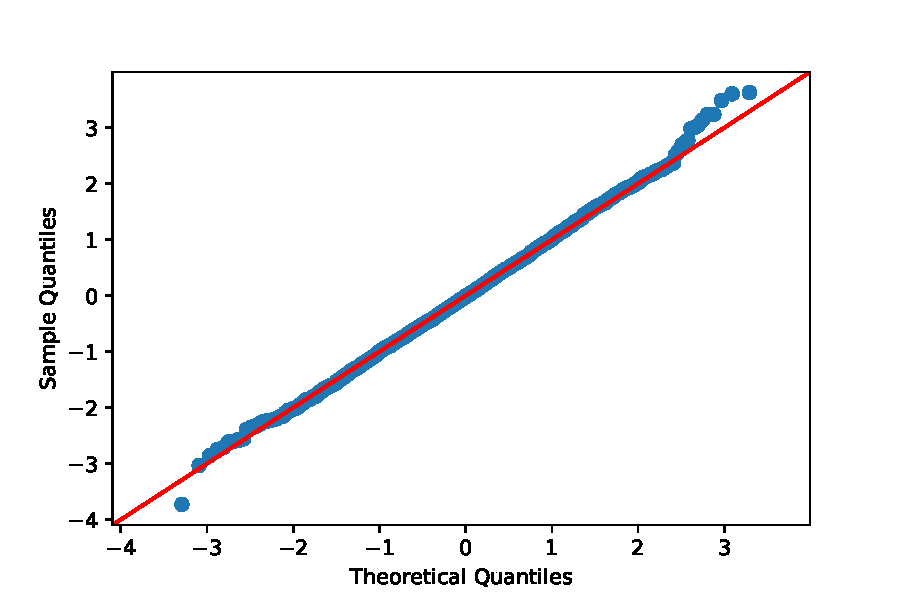
\includegraphics[width=8cm]{obrazek22a.pdf}
				}
				\subfigure{
					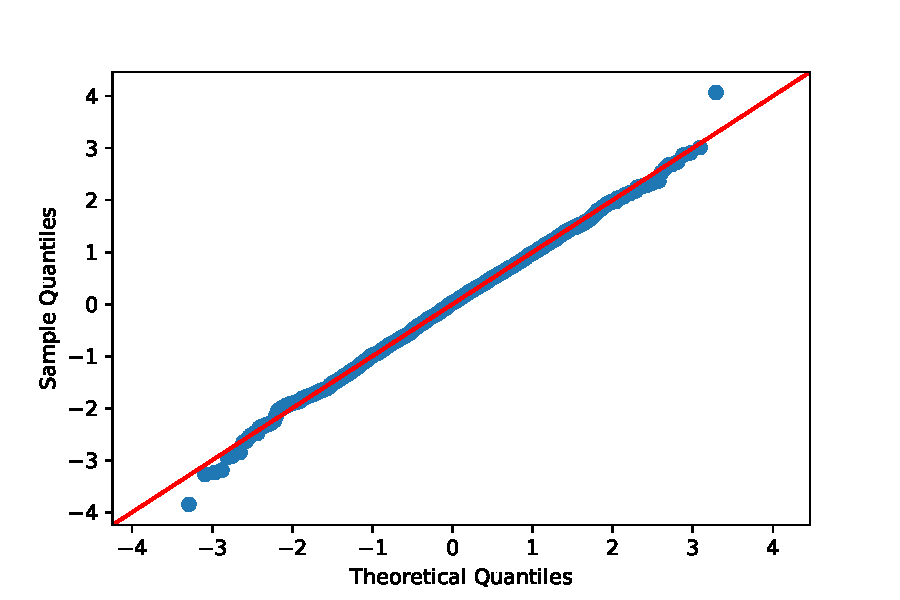
\includegraphics[width=8cm]{obrazek22b.pdf}
				}
				\caption{Gęstości X i Y dla 1000 losowań}
			\end{center}
		\end{figure}
	
		\textbf{Wnioski:}
		
		Metoda ta nie jest za bardzo optymalna, ponieważ musimy wygenerować wartości funkcji trygonometrycznej. Jednak jak możemy zauważyć po porównaniu - gęstości się pokrywają, a więc metoda jest prawidłowo zaimplementowana.
		
		\item\textbf{Metoda biegunowa}\\
		
		Metoda ta jest dość podobna do metody Boxa - M\"{u}llera. Rozpatrywanym obszarem jest koło jednostkowe, tylko tym razem weźmiemy rozkład wektora $(V_{1}, V_{2})$, gdzie:
		$$V_{1} = R\cos{\theta}$$
		$$V_{2} = R\sin{\theta}$$
		$$R = V_{1}^2 + V_{2}^2$$
		Po policzeniu dystrybuanty R i prawdopodobieństwa, że $P(R^2 \le r, \alpha \le a)$, gdzie a = const., otrzymujemy, że $\alpha$ i $R^2$ mają rozkład:
		$$R^2\sim U(0,1)$$
		$$\alpha \sim U(0,2\pi)$$
		Następnie, korzystając z wyliczonych wyżej zmiennych X i Y w metodzie Boxa - M\"{u}llera, możemy podstawić $R^2$ i $\alpha$ odpowiednio za argument logarytmu oraz funkcji trygonometrycznej. W wyniku powyższego działania otrzymujemy następujące zmienne:
		$$X = \sqrt{\frac{-2\log{R^2}}{R^2}}V_{1}$$
		$$Y = \sqrt{\frac{-2\log{R^2}}{R^2}}V_{2}$$
		
		\textbf{Algorytm:}
		\begin{enumerate}
			\item Generuj $V_{1}\sim U(-1,1),V_{2}\sim U(-1,1)$ 
			\item Wyznacz $R^2 = V_{1}^2 + V_{2}^2$
			\item Jeśli $R^2 > 1$ to wróć do a)
			\item wstaw wyliczoną wartość do wyżej wyznaczonej zmiennej X i Y
		\end{enumerate}
		\textbf{Przykładowe implementacje:}
		
		Najpierw pokażamy losowy rozkład powyższej metody dla próby różnej długości:
		\begin{figure}[h]
			\begin{center}
				\subfigure{
					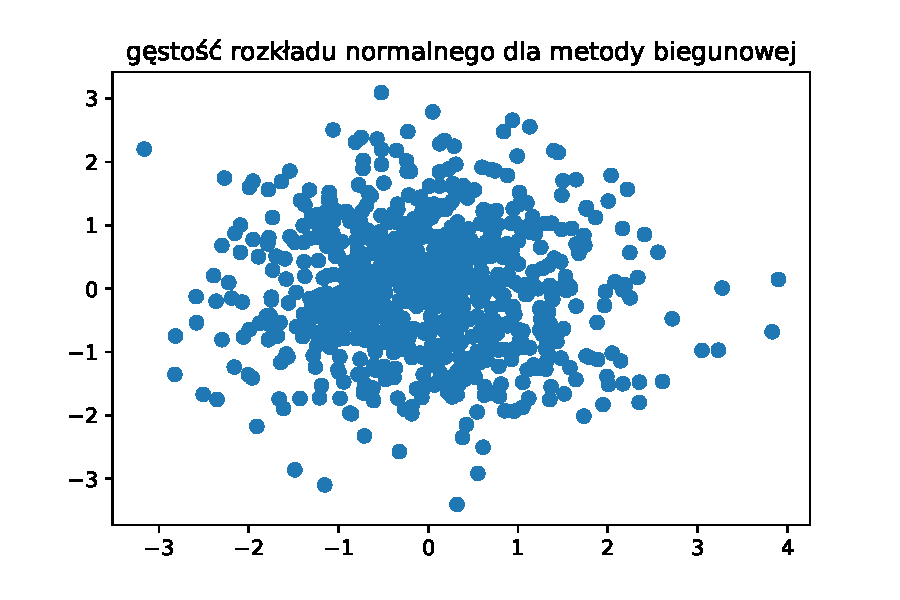
\includegraphics[width=8cm]{obrazek13a.pdf}
				}
				\subfigure{
					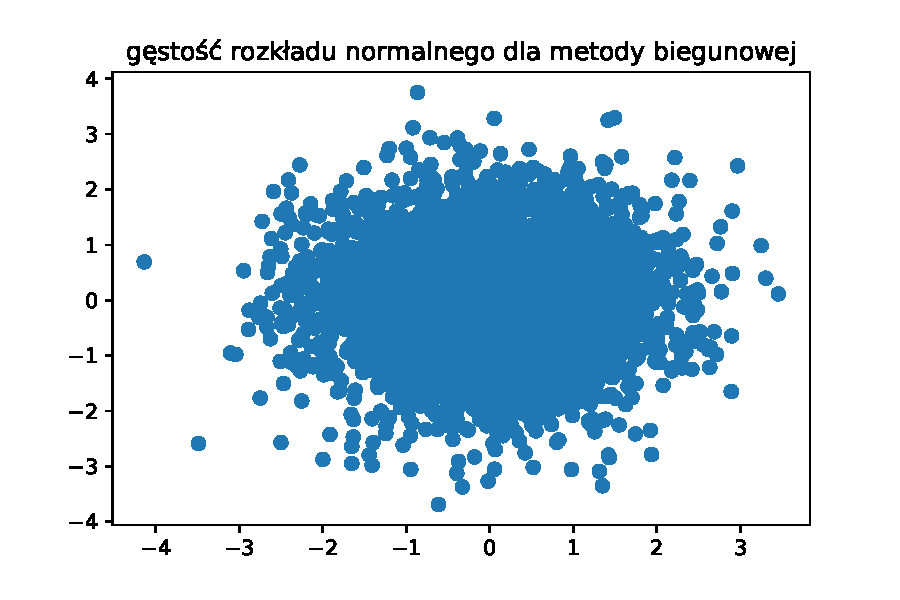
\includegraphics[width=8cm]{obrazek13b.pdf}
				}
				\caption{Gęstości X i Y dla 1000 losowań}
				\caption{Gęstości X i Y dla 5000 losowań}
			\end{center}
		\end{figure}
		Porównamy gęstość empiryczną i teoretyczną:
		\begin{figure}[h]
			\begin{center}
				\subfigure{
					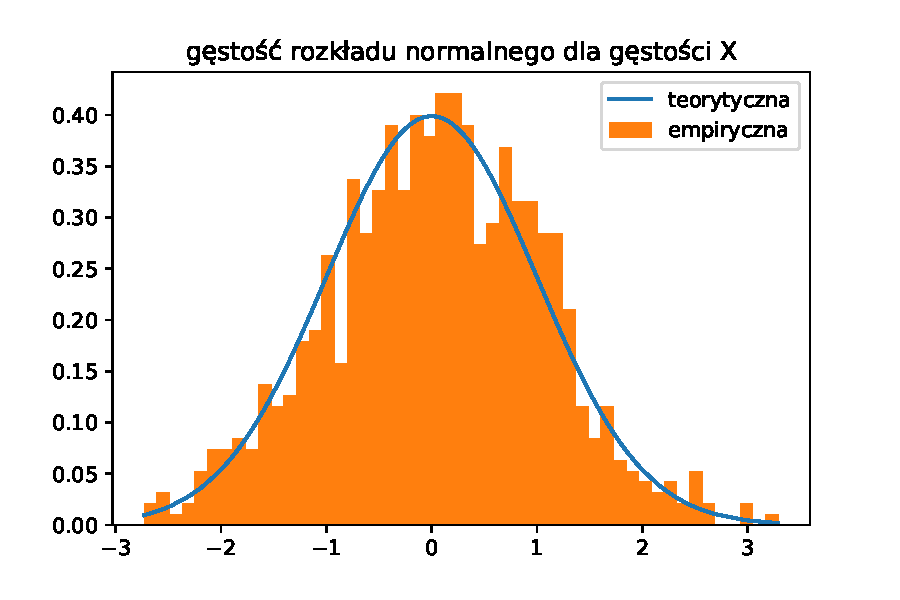
\includegraphics[width=8cm]{obrazek14a.pdf}
				}
				\subfigure{
					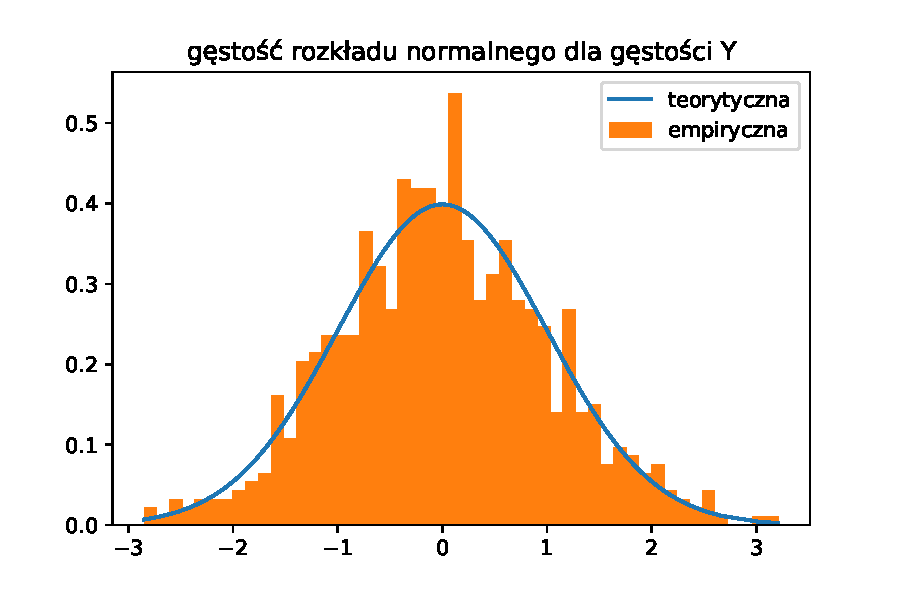
\includegraphics[width=8cm]{obrazek14b.pdf}
				}
				\caption{Gęstości X i Y dla 1000 losowań}
			\end{center}
		\end{figure}
		\begin{figure}[h]
			\begin{center}
				\subfigure{
					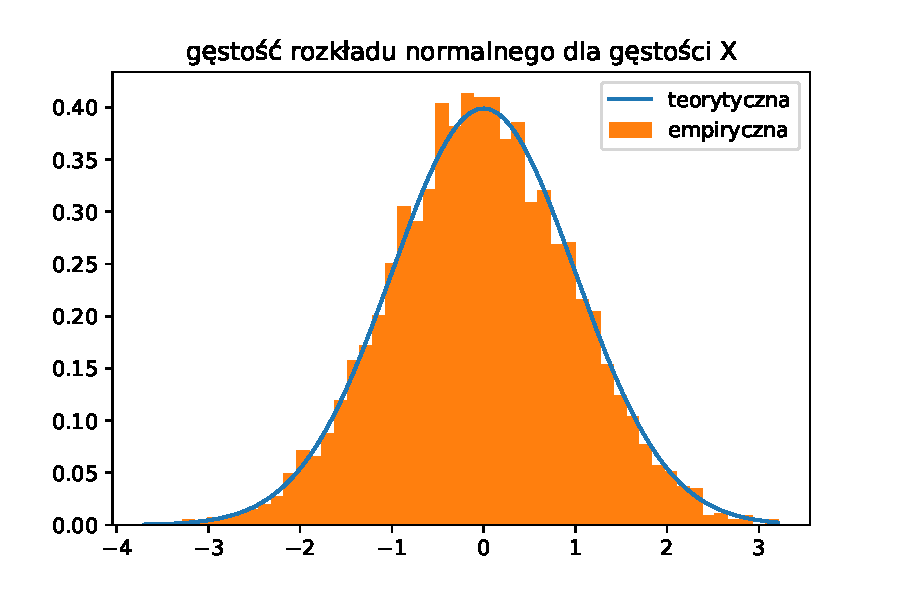
\includegraphics[width=8cm]{obrazek15a.pdf}
				}
				\subfigure{
					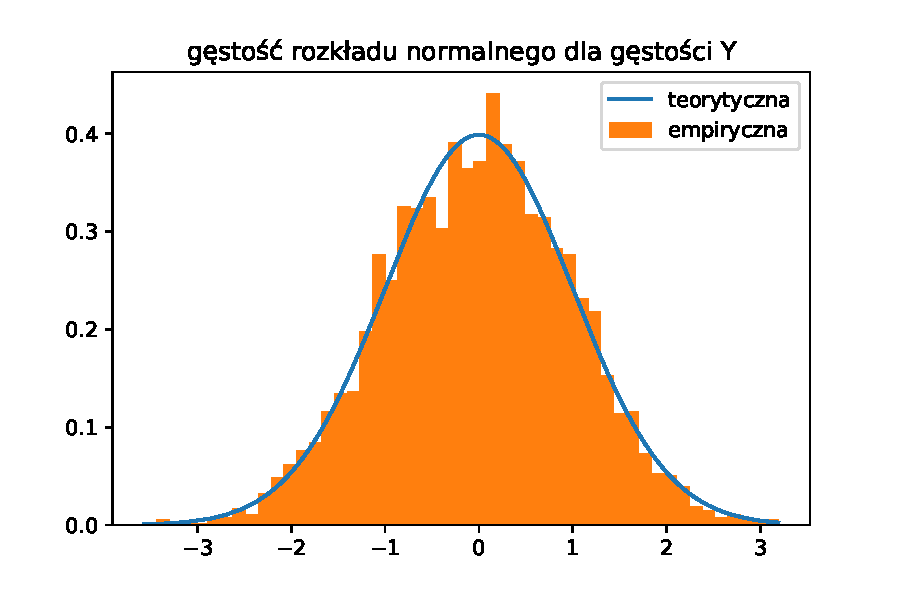
\includegraphics[width=8cm]{obrazek15b.pdf}
				}
				\caption{Gęstości X i Y dla 5000 losowań}
			\end{center}
		\end{figure}
		I sprawdzenie poprawności naszej metody dla wykresu normalnego:
		\begin{figure}[h]
			\begin{center}
				\subfigure{
					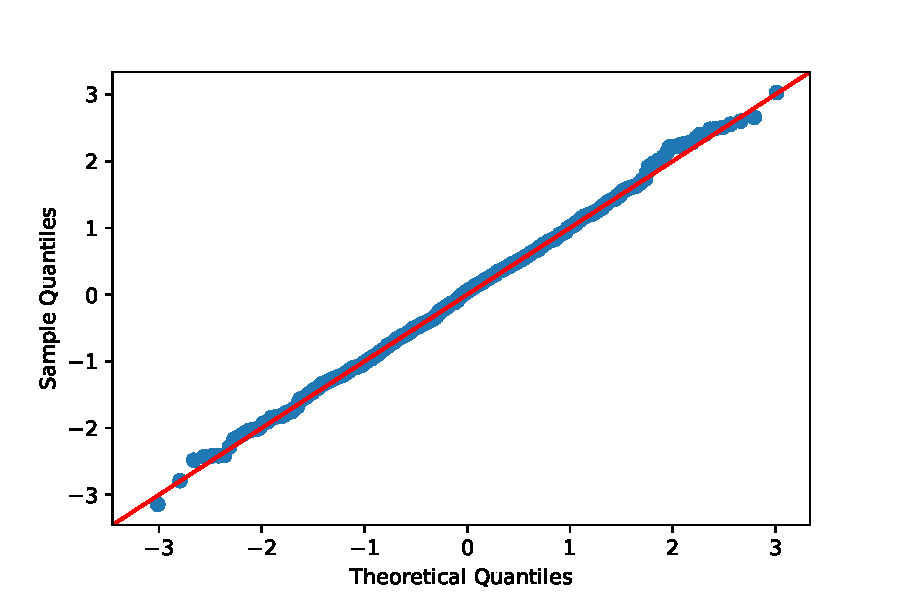
\includegraphics[width=8cm]{obrazek16a.pdf}
				}
				\subfigure{
					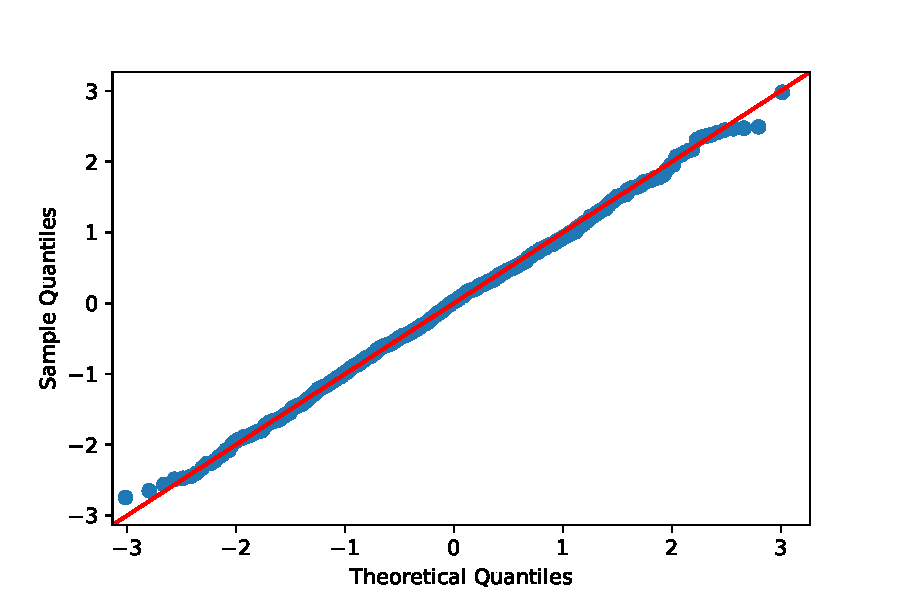
\includegraphics[width=8cm]{obrazek16b.pdf}
				}
				\caption{Gęstości X i Y dla 1000 losowań}
			\end{center}
		\end{figure}
		\begin{figure}[h]
			\begin{center}
				\subfigure{
					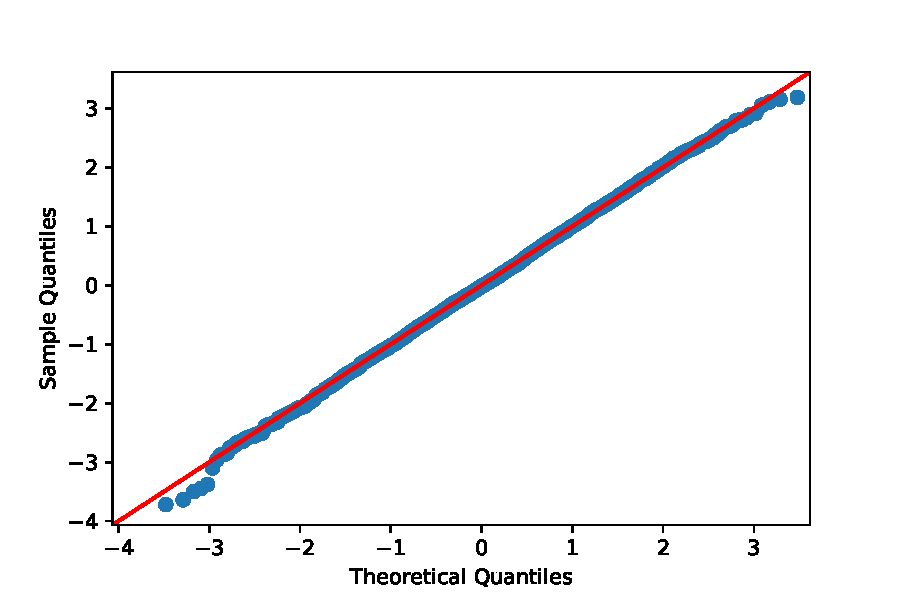
\includegraphics[width=8cm]{obrazek17a.pdf}
				}
				\subfigure{
					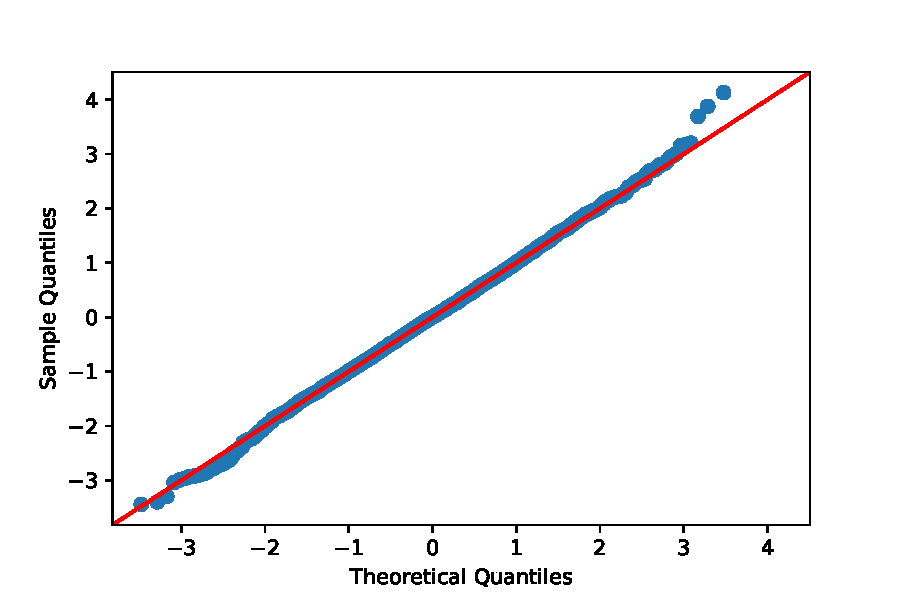
\includegraphics[width=8cm]{obrazek17b.pdf}
				}
				\caption{Gęstości X i Y dla 5000 losowań}
			\end{center}
		\end{figure}
	
		To samo dla dystrybuant:
		
		\begin{figure}[h]
			\begin{center}
				\subfigure{
					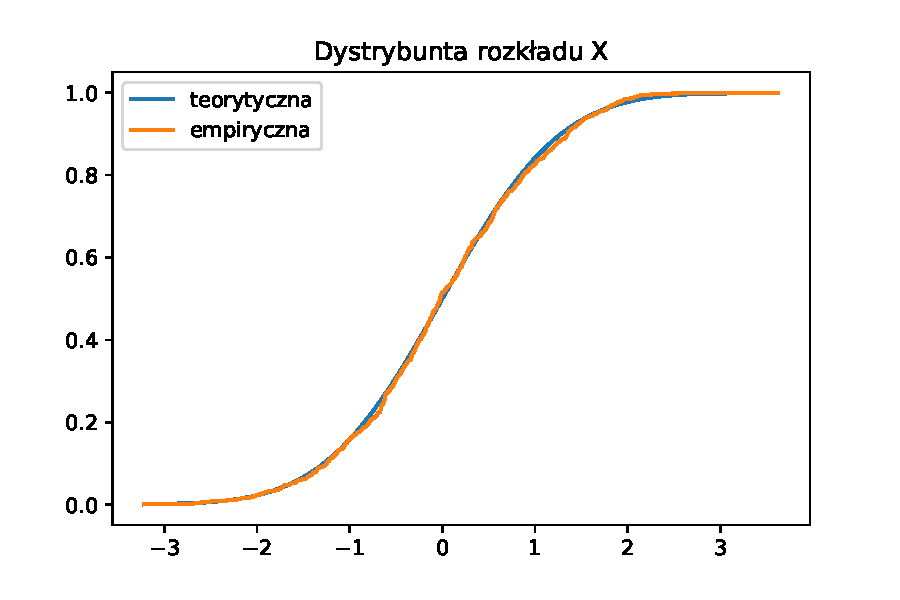
\includegraphics[width=8cm]{obrazek20a.pdf}
				}
				\subfigure{
					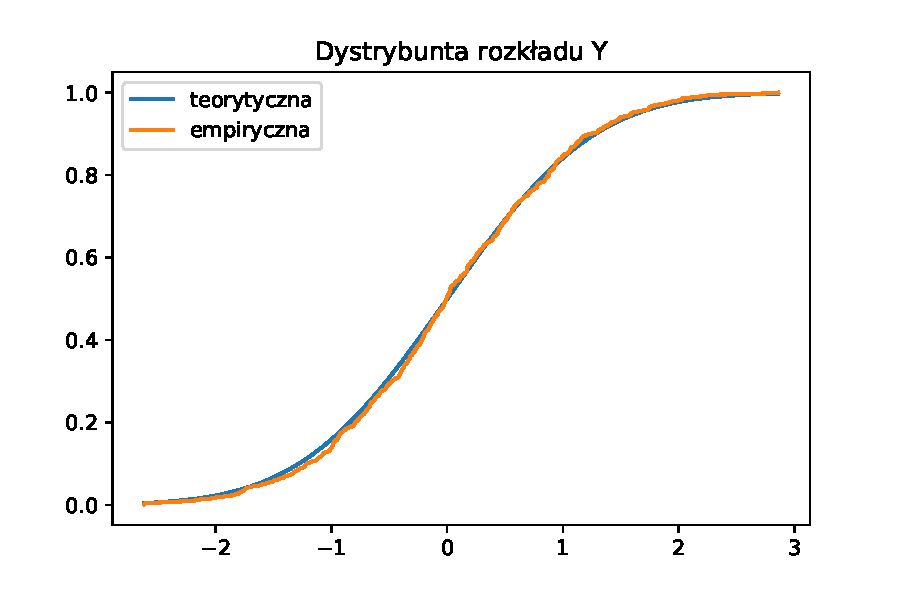
\includegraphics[width=8cm]{obrazek20b.pdf}
				}
				\caption{dla 1000 losowań}
			\end{center}
		\end{figure} 
		
		\begin{figure}[h]
			\begin{center}
				\subfigure{
					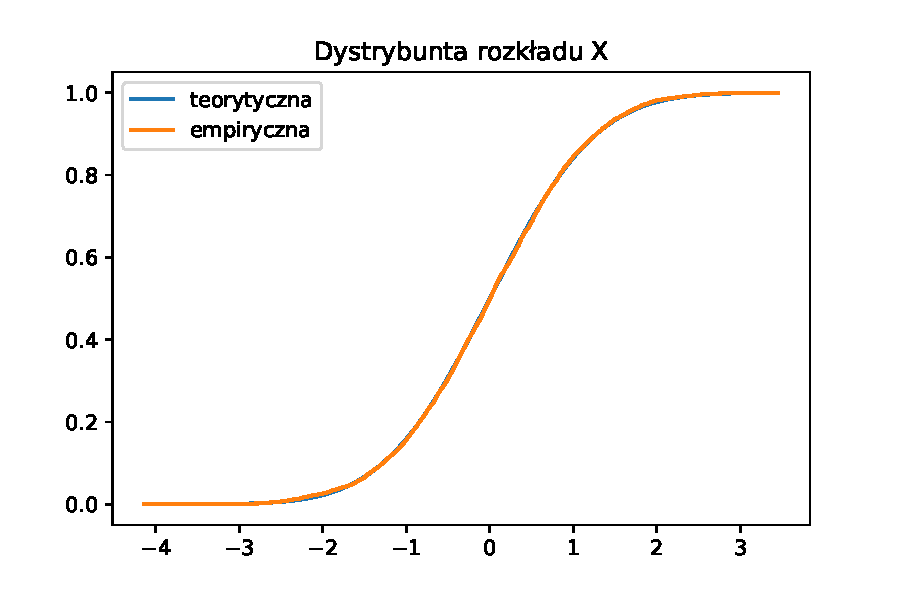
\includegraphics[width=8cm]{obrazek21a.pdf}
				}
				\subfigure{
					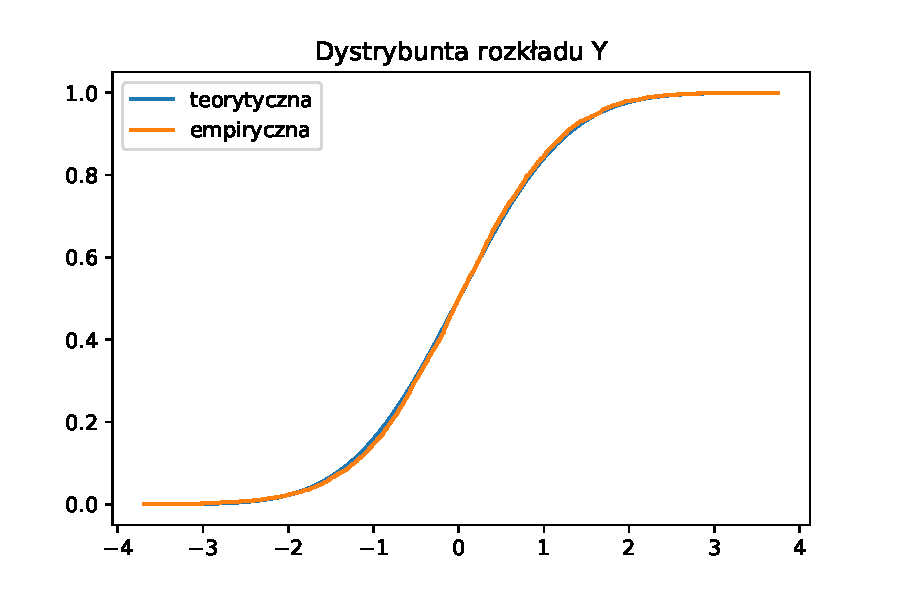
\includegraphics[width=8cm]{obrazek21b.pdf}
				}
				\caption{dla 5000 losowań}
			\end{center}
		\end{figure} 
	
		\textbf{Wnioski:}
		
		Metoda biegunowa jest szybsza i efektywniejsza od metody Boxa - M\"{u}llera. Widzimy również, że gęstości oraz dystrybuanty rozkładów X i Y, pokrywają się z rozkładem normalnym, co oznacza, że nasza implementacja jest poprawna. Im większa miara próby rozkładu, tym wykresy są bardziej zbliżone do wbudowanego rozkładu normalnego.
		
	\end{enumerate}
\end{document}